\documentclass[12pt,aspectratio=169]{beamer}
\usecolortheme{udec}
\usetheme{udec}
\usepackage{graphicx}
\graphicspath{{img/},{slides/}}
\usepackage{pgffor}
\usepackage{tikz}
\usepackage{fontspec}
\usepackage{gelasio}
\usefonttheme{serif}
\setmainfont{Gelasio}
\usepackage{polyglossia}
\setmainlanguage{spanish}
\setbeameroption{show notes on second screen=bottom}

\newcommand<>{\fullsizegraphic}[1]{
	\begin{tikzpicture}[remember picture,overlay]
	\node[at=(current page.center)] {
		\includegraphics{#1}
	};
	\end{tikzpicture}
}

\title{Establecimiento de protocolo de comunicación entre X-Plane y microcontroladores externos}
\subtitle{Proyecto de ingeniería aeroespacial}
\author{Por Germán Quijada}
\institute{Profesor guía:\\Bernardo Hernández}

\begin{document}
\begin{frame}[noframenumbering]
\maketitle
\end{frame}

\begin{frame}{Contenidos}
\tableofcontents
\end{frame}

%% Introducción
\section{Concepto}
\begin{frame}{Concepto}
En el simulador de vuelo del laboratorio de técnicas aeroespaciales, establecer un \emph{protocolo de comunicación} entre el software de simulación \emph{X-Plane} y \emph{microcontroladores externos}.
\note{
En el simulador de vuelo del laboratorio de técnicas aeroespaciales, establecer un protocolo de comunicación entre el software de simulación X-Plane y microcontroladores externos

Se define que en el laboratorio de técnicas aeroespaciales de la universidad de Concepción solo para acotar el problema, pero en la práctica no hay razón para que lo implementado en el laboratorio no funcione en otro computador personal
}
\end{frame}

\section{Actores en la comunicación}
\begin{frame}[noframenumbering]
\sectionpage
\note{
Analicemos un poco el problema desde lo más básico, que es X-Plane y que es un microcontrolador y por qué se querría establecer comunicación entre ellos
}
\end{frame}

\subsection{X-Plane}
\begin{frame}{X-Plane}
\begin{itemize}
	\item Software de simulación de vuelo
	\item<2-> Utilizado en entornos de entrenamiento certificados\footnotemark
	\item<3-> Herramienta ingenieril\footnotemark
	\item<4-> Funcionalidad agregada con plug-ins
	\item<5-> Interfaz de comunicación UDP
\end{itemize}
\only<2->{
	\footnotetext[1]<2->{\url{https://x-plane.helpscoutdocs.com/article/31-faa-certification}}
	\footnotetext[2]<3->{\url{https://www.x-plane.com/desktop/meet\_x-plane}}
}
\note<1>{
	X-Plane es un simulador de vuelo que destaca por sus físicas de vuelo realistas y es popular tanto para entusiastas de la aviación como para pilotos en entrenamiento.
}
\note<2>{
	En conjunto con el hardware apropiado, X-Plane cumple con los requisitos y normas de simulación de vuelo necesarios para su uso en entrenamiento de pilotos y otras aplicaciones relacionadas con la aviación.
}
\note<3>{
	Debido a lo realista del modelo de vuelo, X-Plane puede evaluar el rendimiento de nuevas configuraciones de aeronaves, realizar análisis de vuelo, simular condiciones específicas y validar conceptos antes de la construcción física.
}
\note<4>{
	X-Plane cuenta con herramientas de desarrollo para crear plug-ins personalizados y en internet hay muchos publicados por terceros, esta podría ser una forma de abordar la implementación del protocolo.
}
\note<5>{
	Otra forma de establecer comunicación es por medio de la interfaz UDP integrada en el simulador, sin embargo este medio está orientado a desarrolladores y no es fácil de usar.
}
\end{frame}

\begin{frame}
\centering
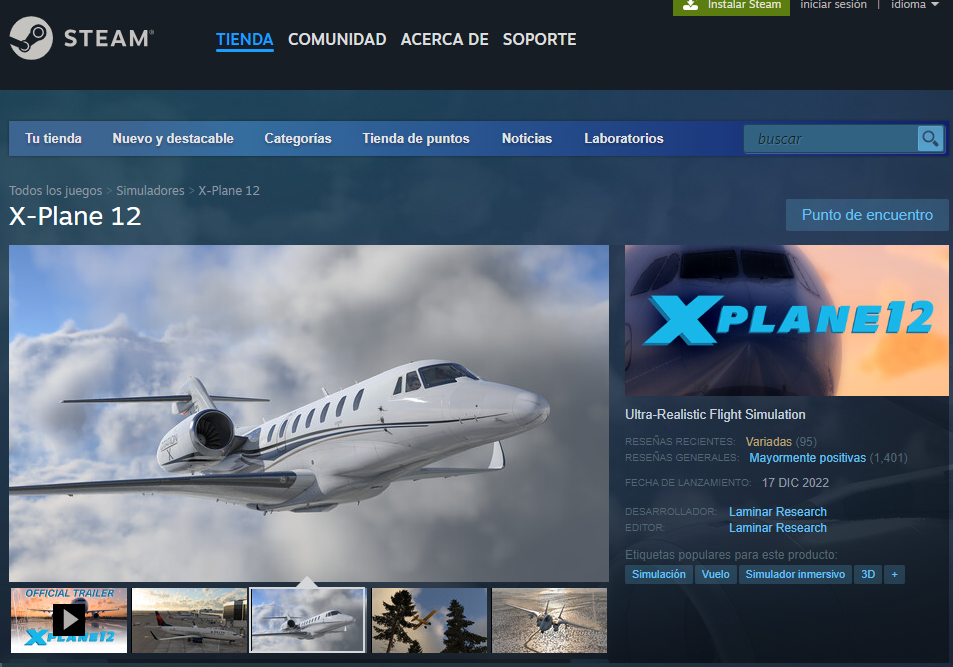
\includegraphics[width=0.8\textwidth]{xplane-steam.png}
\end{frame}

\subsection{Microcontrolador}
\begin{frame}{Microcontroladores}
\begin{itemize}
	\item Pequeños dispositivos electrónicos integrados
	\item<2-> Especializados
	\item<3-> Interfaces estandarizadas ($I^2C$, Serial, UART)
	\item<4-> Baratos
\end{itemize}
\note<1>{
	El microcontrolador es un dispositivo electrónico integrado que en sus formas más simples combina una unidad de procesamiento, memoria y alguna interfaz de entrada y salida de señales. Se podría decir que es como un computador, pero muy muy pequeño y utilizados para una sola tarea especifica.
}
\note<2>{
	Una vez programado se tiene mucha seguridad que en cada encendido el microcontrolador ejecutara las órdenes tal cual fueron escritas y nada más.
}
\note<3>{
	Por lo general los microcontroladores habilitan una o más interfaces de comunicación con otros microcontroladores o cualquier dispositivo que implemente la misma interfaz. Algunos ejemplos son I2C, Serial y UART entre muchos otros.
}
\note<4>{
	Y por lo último los microcontroladores al no presentar funciones más complejas pueden llegar a ser muy baratos sin necesidad de comprometer alguna funcionalidad. En la práctica la condicional para elegir entre un microcontrolador u otro va a ser las funciones de cada uno en vez del precio. 
}
\end{frame}

\begin{frame}
\begin{columns}
\begin{column}{0.45\textwidth}{
	\begin{figure}[t]
		\centering
		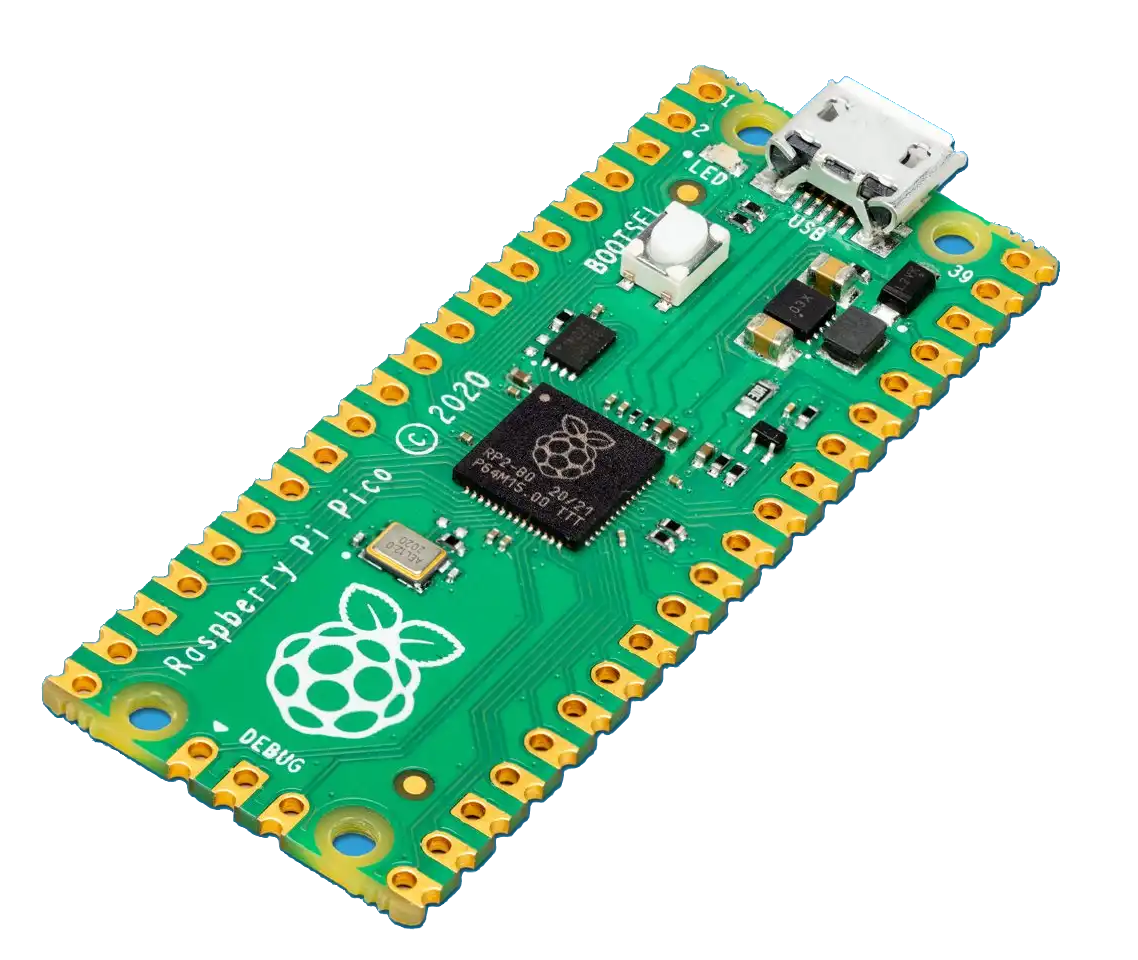
\includegraphics[width=0.6\textwidth]{raspberry-pi-pico.png}
		\caption{Raspberry Pi Pico\footnotemark}
\end{figure}
}
\end{column}
\begin{column}{0.45\textwidth}{
	\begin{figure}[t]
		\centering
		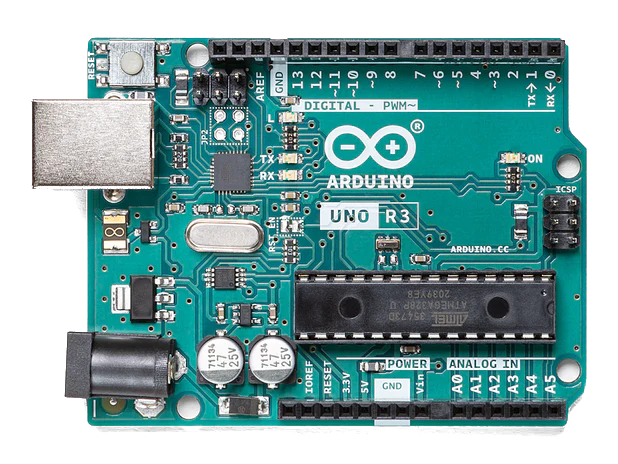
\includegraphics[width=0.6\textwidth]{arduino-uno.png}
		\caption{Arduino UNO\footnotemark}
	\end{figure}
}
\end{column}
\end{columns}
\footnotetext[1]{\url{https://www.raspberrypi.com/products/raspberry-pi-pico/}}
\footnotetext[2]{\url{https://store.arduino.cc/products/arduino-uno-rev3}}
\end{frame}

\begin{frame}{Integración X-Plane - Microcontrolador}
\begin{itemize}
	\item <2-> Desarrollar sistemas de control
	\item <3-> Evaluar rendimiento de maniobras o en misiones
	\item <4-> Código portable
\end{itemize}
\note<1>{
	Veamos brevemente algunas aplicaciones en que la comunicación entre los actores podría ser beneficiosa
}
\note<2>{
	Con la capacidad de analizar y responder al estado de la aeronave es posible desarrollar algoritmos de control o de piloto automático.
}
\note<3>{
	Gracias a que se trabaja con simulaciones, es posible manipular el estado arbitrariamente y ejecutar maniobras de manera iterativa reiniciándolas una y otra vez con fines de optimización
}
\note<4>{
	Para esta y todas las aplicaciones, el código al correr en un microcontrolador será completamente portable y podrá ser reimplementado a cualquier otro sistema o aeronave real mientras se pueda acceder a una interfaz de datos.
}
\end{frame}

%% Diseño del protocolo
\section{Diseño de protocolo}
\begin{frame}[noframenumbering]
\sectionpage
\end{frame}

\subsection{Diseño preliminar}
\begin{frame}{Diagrama preliminar}
\foreach \n in {1,...,5}{
	\only<\n>{\fullsizegraphic{diagrama-preliminar-step-\n.pdf}}
}
\end{frame}

\begin{frame}{Condiciones de diseño}
\begin{itemize}
	\item<2-> En el simulador del laboratorio de técnicas aeroespaciales
	\begin{itemize}
		\item<3-> Funcionar con X-Plane 9 y 10
	\end{itemize}
	\item<4-> Funcionar en microcontroladores Arduino y Raspberry Pi Pico
	\item<5-> Accesible para usuarios con poca experiencia programando
\end{itemize}
\end{frame}

\subsection{Soluciones existentes}
\begin{frame}[noframenumbering]
\subsectionpage
\end{frame}

\begin{frame}{NASA X-Plane Communications Toolbox}
\begin{figure}[t]
	\centering
	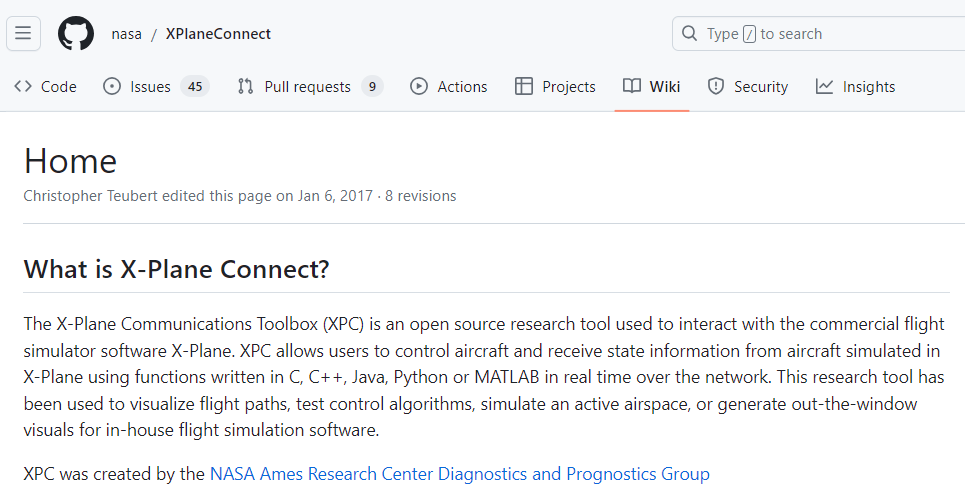
\includegraphics[width=0.9\textwidth]{nasa.png}
	\footnotemark
\end{figure}
\footnotetext{\url{https://github.com/nasa/XPlaneConnect/wiki}}
\end{frame}

\begin{frame}{NASA X-Plane Communications Toolbox}
\fullsizegraphic{diagrama-nasa-step-1.pdf}
\end{frame}

\begin{frame}{Interfaz UDP integrada en X-Plane}
\begin{figure}[t]
	\centering
	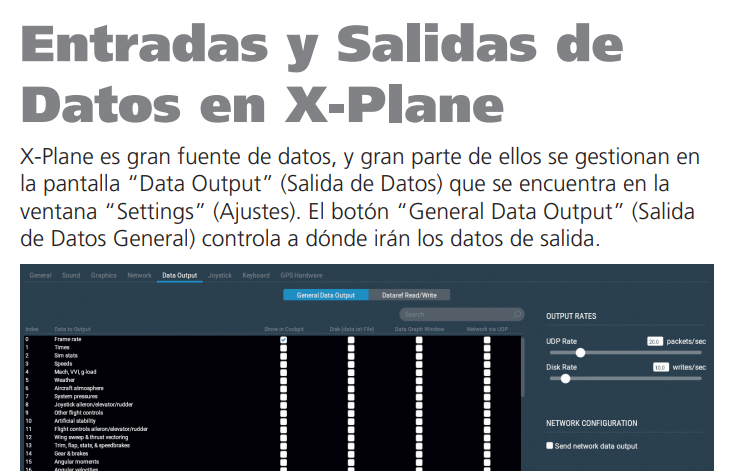
\includegraphics[width=0.7\textwidth]{xplane-udp.png}
	\footnotemark
\end{figure}
\footnotetext{\url{https://www.x-plane.com/wp-content/uploads/2017/04/Manual_XPlane11_sp_web.pdf}}
\end{frame}

\begin{frame}{Interfaz UDP integrada en X-Plane}
\fullsizegraphic{diagrama-nasa-step-1.pdf}
\end{frame}

\begin{frame}{\large Flight Simulator Universal Inter-Process Communication}
\begin{figure}[t]
	\centering
	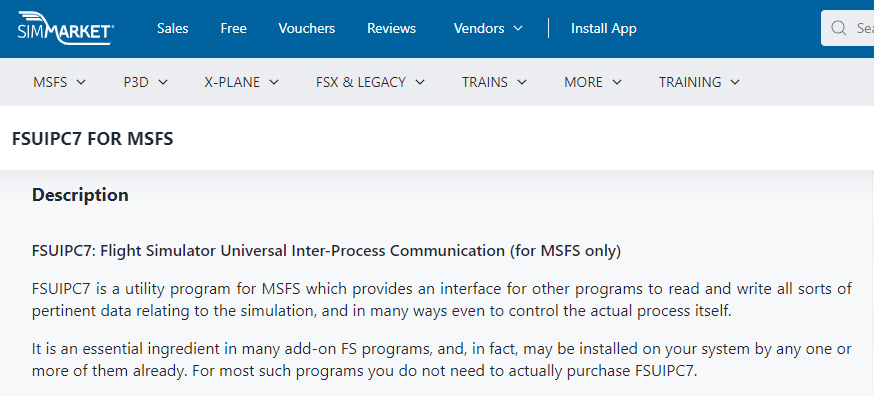
\includegraphics[width=0.9\textwidth]{fsuipc.png}
	\footnotemark
\end{figure}
\footnotetext{\url{https://secure.simmarket.com/john-dowson-fsuipc7-for-msfs.phtml}}
\end{frame}

\begin{frame}{\large Flight Simulator Universal Inter-Process Communication}
	\fullsizegraphic{diagrama-fsuipc-step-1.pdf}
\end{frame}

\subsection{Diseño final}
\begin{frame}[noframenumbering]
\subsectionpage
\end{frame}

\begin{frame}{Consideraciones}
\begin{itemize}
	\item Condiciones de diseño
	\begin{itemize}
		\item<2-> Todas las opciones funcionan con X-Plane 9 y 10
		\item<3-> Muy pocas alternativas diseñadas para microcontrolador
		\item<4-> Las soluciones no son amigables
	\end{itemize}
	\item<5-> Decisiones tomadas
	\begin{itemize}
		\item<6-> Crear software intermediario personalizado
		\item<7-> Construir sobre FSUIPC
	\end{itemize}
\end{itemize}
\end{frame}

\begin{frame}{Diagrama}
	\fullsizegraphic{diagrama-fssp-step-1.pdf}
\end{frame}

\begin{frame}{Programa intermediario}
\begin{itemize}
	\item Comunicación con simulador por plug-in FSUIPC
	\item Abre dos canales de comunicación a equipos externos
	\begin{itemize}
		\item UDP (Red local)
		\item Serial (USB)
	\end{itemize}
	\item<2-> Escrito en C++
\end{itemize}
\end{frame}

\begin{frame}{Protocolo}
\begin{itemize}
	\item Strings y secuencias de bytes enviables por UDP y serial

	\item Las strings se utilizan para establecer cuantas y cuales variables se enviaran y recibiran posteriormente en secuencias de bytes, ademas del envio de comandos puntuales

	\item Las secuencias de bytes contienen la información establecida por las strings, usualmente variables que necesitan ser revisadas con frecuencia como el estado de la aeronave o el envio de comandos para el control
\end{itemize}
\end{frame}

\section{Implementación}
\begin{frame}[noframenumbering]
\sectionpage
\end{frame}

\subsection{Comunicación}
\begin{frame}{Software intermediario - X-Plane}
\begin{itemize}
	\item Creado con la libreria de desarrollo para plug-ins de FSUIPC
\end{itemize}
\end{frame}

\begin{frame}{Software intermediario - Microcontrolador}
\begin{itemize}
	\item Creado con libreria general para comunicación Serial
	\item "" para comunicación por red (Windows Sockets 2)
\end{itemize}
\end{frame}

\subsection{Protocolo}
\begin{frame}{Comandos básicos}
\begin{itemize}
	\item Monitorear variables
	\item Controlar variables
\end{itemize}
\end{frame}

\subsection{QoL}
\begin{frame}{Funcionalidad QoL}
Interfaz grafica que muestra si esta conectado con el simulador, con el microcontrolador, los mensajes que recibe y un terminal para probar el envio y recepcion de mensajes
\end{frame}

\begin{frame}
\begin{figure}[t]
	\centering
	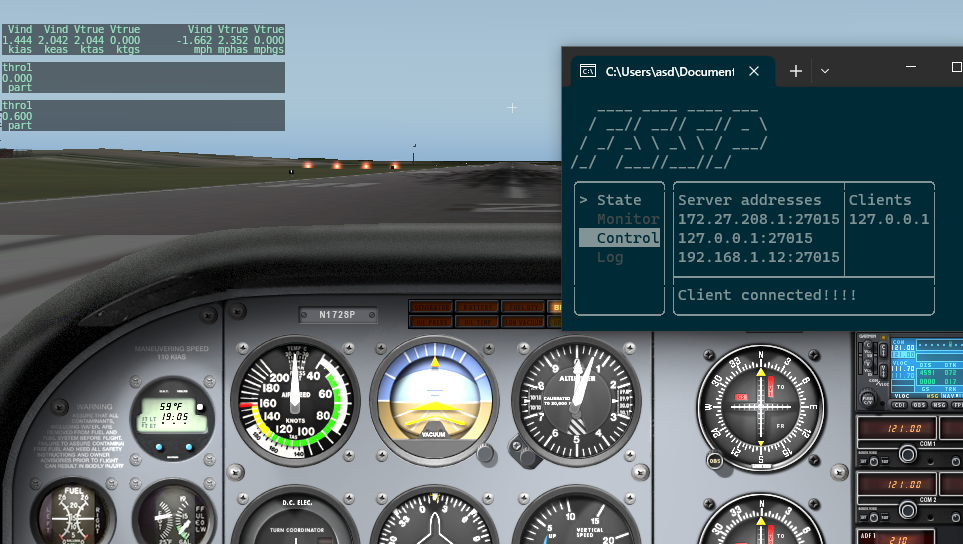
\includegraphics[width=0.8\textwidth]{fssp.png}
\end{figure}
\end{frame}

\section{Conclusión}
\begin{frame}[noframenumbering]
\sectionpage
\end{frame}

\begin{frame}{Objetivos}
Se establece el protocolo de comunicación entre el sistema 
\end{frame}

\begin{frame}[noframenumbering]
\centering
\Large \textbf{Gracias por su atención}
\end{frame}

\end{document}